

\section{Мобильный робот в форме эллипсоида}
\small

%\begin{frame}[plain, noframenumbering]
%	\begin{center}
%		\Huge
%		\todo{Мобильный робот в форме эллипсоида}
%	\end{center}
%\end{frame}

\begin{frame}
\frametitle{Актуальность}
	Способы перемещения роботов в жидкости:
	\begin{itemize}
		\item Гребные винты. Самый распространенный способ передвижения.
		\item Изменение формы тела. 
		\item Реакивный привод.
		\item Действие внутренних механизмов.		
	\end{itemize}	

	\begin{minipage}[t]{0.47\linewidth}
		\center{\includegraphics[height=24mm]{ScrewRobot.png}}
	\end{minipage}
	\hfill
	\begin{minipage}[t]{0.47\linewidth}
		\center{\includegraphics[height=24mm]{FishRobot.png}}
	\end{minipage}	
	\vspace{3mm}
	
	\begin{minipage}[t]{0.47\linewidth}
		\center{\includegraphics[height=22mm]{JatsunRobot.png}}
	\end{minipage}
	\hfill
	\begin{minipage}[t]{0.47\linewidth}
		\center{\includegraphics[height=22mm]{TolikRobot.png}}
	\end{minipage}

\end{frame}	
	

%\begin{frame}
%\frametitle{Актуальность}
%	
%	Преимущества и недостатки использования гребных винтов
%	\begin{minipage}[t]{0.49\linewidth}
%		Преимущества
%		\begin{itemize}
%			\item Теория передвижения хорошо изучена.
%			\item Относительная простота конструкции
%			\item Скорость передвижения
%		\end{itemize}
%	\end{minipage}
%	\hfill
%	\begin{minipage}[t]{0.49\linewidth}
%		Недостатки
%		\begin{itemize}
%			\item Наличие гидродинамических шумов.
%			%\item Низкая маневренность.
%			\item Повреждение окружающей микрофлоры.
%			\item Выход вала с гребным винтом требует герметизации.
%		\end{itemize}
%	\end{minipage}
%
%	\vspace{2mm}
%	
%	Особенности водных роботов, перемещающихся за счет движения внутренних масс и/или вращения внутренних роторов%, у которых форма оболочки робота остается неизменной.
%	%Преимущества данного типа движения:
%		\begin{itemize}
%			\item отсутствие приводных элементов, взаимодействующих со средой;
%			\item возможность полной гидроизоляции;
%			%\item низкий уровень гидродинамического шума при передвижении;
%			%\item повышенная маневренность.
%		\end{itemize}
%		
%
%
%	%В данной работе рассматриваются роботы без внешних приводных элементов, перемещающиеся в жидкости за счет вращения внутренних роторов.
%
%\end{frame}

\begin{frame}
\frametitle{Основные работы по тематике исследования}
	
	\begin{itemize}
		\item Модель в рамках идеальной жидкости, учитывающая эффект присоединенных масс. Показана возможность неограниченного продвижения при наличии анизотропии присоединенных масс. В.В. Козлов, С.М. Рамоданов, Д.А. Онищенко.
	\end{itemize}

		\begin{minipage}[t]{0.6\linewidth}
			\vspace{-13mm}
			\begin{itemize}
				\item Модели движения в идеальной жидкости с заданным законом сопротивления. Ф.Л. Черноусько, Н.Н. Болотник, С.Ф. Яцун.
			\end{itemize}
		\end{minipage}
		\hfill
		\begin{minipage}[t]{0.30\linewidth}
			\center{\includegraphics[height=13mm]{ChernouskoRobot.png}}
		\end{minipage}	
	
	\begin{itemize}
		\item Численное моделирование гидродинамики движущегося объекта на основе совместного решения уравнений Навье-Стокса и уравнений динамики твердого тела. В.А. Тененев, С.М. Рамоданов, Е.В. Ветчанин.
		
		\item Влияние вязкости на самопродвижение твердого тела с движущейся внутри него массой. S. Childress
		
		\item Исследование движения роботов различной формы и конструкции, приводимые в движение внутренними механизмами. Е.В. Ветчанин, И.С. Мамаев, А.А. Килин.
		
		%\item Подробный обзор работ, посвященных движению твердого тела в жидкости, используя внутренние механизмы:
		
		%Ветчанин Е. В., Килин А. А., Управляемое движение твердого тела с внутренними механизмами в идеальной несжимаемой жидкости, Труды Математического института имени В. А. Стеклова, 2016, т. 295, с. 321-351
		%\item Экспериментальные работы: А.А. Килин, А.И. Кленов, В.А. Тененев. Управление движением тела с помощью внутренних масс в вязкой жидкости.		
	\end{itemize}

\end{frame}

\begin{frame}
\frametitle{Экспериментальные работы.}

	\begin{itemize}
		\item А.А. Килин, А.И. Кленов, В.А. Тененев. Управление движением тела с помощью внутренних масс в вязкой жидкости.
		\begin{figure}[h]
			\center{\includegraphics[height=25mm]{TolikRobot.png}}
		\end{figure}
		
		\item Работы Ф. Таллапрагада с соавторами -- сложная модель движения с вихреобразованием.
		\begin{figure}[h]
			\center{\includegraphics[height=25mm]{TallapragadaRobot.png}}
		\end{figure}
		
	\end{itemize}

\end{frame}


\begin{frame}%[allowframebreaks]
	\frametitle{Математическая модель. Уравнения движения}
		\qquad Рассмотрим систему, состоящую из жесткой внешней оболочки и трех внутренних роторов.
		
		\begin{minipage}[t]{0.4\linewidth}
			\begin{figure}[h]
				\begin{center}
					\includegraphics[height=0.8\linewidth]{BPR_Scheme.png} %Shell.eps %BPR_Scheme.png				
				\end{center}
			\end{figure}	
		\end{minipage}
		\hfill
		\begin{minipage}[t]{0.57\linewidth}
			$O x y z$ -- неподвижная система координат;
			
			$O_M e_1 e_2 e_3$ -- подвижная система координат;
			
			$\br = \bigl( x,\, y,\, z \bigr)$ -- координаты геометрического центра оболочки;
			
			${\bal}$, ${\bbe}$, ${\bga}$ -- орты неподвижных осей $O x y z$, спроецированные на подвижные оси $e_1$, $e_2$, $e_3$;

			$\bV$ и ${\bOm}$ -- скорость центра оболочки и его угловая скорость.
			
		\end{minipage}	
	
	Кинематические соотношения и уравнения эволюции $\bigl( \br,\, {\bbQ} \bigr)$:	
	\begin{minipage}{0.47\linewidth}
		%\vspace{-3mm}
		\begin{gather*}
		\dot{{\bal}} = {\bal} \times {\bOm},\, \dot{{\bbe}} = {\bbe} \times {\bOm},\, \dot{{\bga}} = {\bga} \times {\bOm},\\
		\dot{\br} = {\bbQ}^T \bV.
		\end{gather*}	
	\end{minipage}
	\begin{minipage}{0.47\linewidth}
		\vspace{-3mm}
		\begin{gather}
		\bbQ =\begin{pmatrix}
		\alpha _1 & \beta _1 & \gamma _1\\
		\alpha _2 & \beta _2 & \gamma _2\\
		\alpha _3 & \beta _3 & \gamma _3
		\end{pmatrix}\nonumber \in SO(3)
		\end{gather}
	\end{minipage}
	
	Уравнения движения рассматриваемой системы имеют вид классических уравнений Кирхгофа
	\begin{gather}
	\frac{d}{dt} \biggl( \frac{\partial T}{\partial \bV} \biggr) + {\bOm} \times \frac{\partial T}{\partial \bV}=0, \quad \frac{d}{dt}\biggl( \frac{\partial T}{\partial {\bOm}} \biggr) + {\bOm} \times \frac{\partial T}{\partial {\bOm}} + \bV \times \frac{\partial T}{\partial \bV} = 0 \nonumber
	\end{gather}
	
\end{frame}



\begin{frame}
\frametitle{Уравнения движения}
\begin{itemize}
	
	\item После подстановки кинетической энергии в уравнения Кирхгоффа уравнения движения принимают вид
	\begin{gather*}
	\begin{split}
	{\bbC} \dot{\bV} + {\bbB} \dot{{\bOm}} = & \bigl( {\bbC} \bV + {\bbB} {\bOm} \bigr) \times {\bOm},\\
	{\bbB}^T \dot{\bV} + {\bbI} \dot{{\bOm}} + \dot{\bK}(t) = & \bigl( {\bbB}^T \bV + {\bbI} {\bOm} + \bK(t) \bigr) \times {\bOm} + \bigl( {\bbC} \bV + {\bbB} {\bOm} \bigr) \times \bV = 0
	\end{split}
	\end{gather*}
	
	\item Для полного описания движения системы данные уравнения необходимо дополнить уравнениями эволюции переменных $\bigl( \br,\, {\bbQ} \bigr)$%, которые описываются уравнениями Пуассона 
	и кинематическими соотношениями 
	\begin{gather*}
	\dot{{\bal}} = {\bal} \times {\bOm},\quad \dot{{\bbe}} = {\bbe} \times {\bOm},\quad \dot{{\bga}} = {\bga} \times {\bOm},\quad
	\dot{\br} = {\bbQ}^T \bV.
	\end{gather*}
	
	\item Уравнения в форме импульса и момента импульса:
	\begin{gather*}
	\label{motion_ham}
	\dot{\bP}= \bP \times {\bOm}, \quad \dot{\bM} = \bM \times {\bOm} + \bP \times \bV,
	\end{gather*}	
	где $\bP = \dfrac{\partial T}{\partial \bV}$ и $\bM = \dfrac{\partial T}{\partial {\bOm}}$ 
	
	\item Связь $\bV$ и ${\bOm}$ с $ \bP $ и $\bM  $:
	\begin{gather}
	\label{p_and_M}
	\begin{split}
	\bP = & {\bbC} \bV + {\bbB} {\bOm},\, \quad \bM = {\bbB}^T \bV + {\bbI} {\bOm} + \bK(t),\\
	\bV = & {\bbC}^{-1} \bigl( \bP - {\bbB} {\bOm} \bigr),\, \quad {\bOm} = \bigl({\bbI} - {\bbB}^T {\bbC}^{-1} {\bbB} \bigr)^{-1} \bigl( \bM - \bK(t) - {\bbB}^T {\bbC}^{-1} \bP \bigr)
	\end{split}\nonumber
	\end{gather}
	
\end{itemize}
\end{frame}

\begin{frame}
\frametitle{Первые интегралы}
\begin{itemize}
	
	

	
	\item Уравнения допускают шесть геометрических интегралов движения:
	\begin{gather}
	{\bal}^2={\bbe}^2={\bga}^2=1, \quad \bigl({\bal},\, {\bbe} \bigr) = \bigl({\bal},\, {\bga} \bigr) = \bigl({\bbe},\, {\bga} \bigr) = 0\nonumber
	\end{gather}
	
	\item Уравнения в гамильтоновой форме допускают еще шесть интегралов
	\begin{gather*}
	(\bP,\, {\bal}),\, (\bP,\, {\bbe}),\, (\bP,\, {\bga}),\, (\bM + \br \times \bP,\, {\bal}),\, (\bM + \br \times \bP,\, {\bbe}),\, (\bM + \br \times \bP,\, {\bga}) \label{integrals}
	\end{gather*}
	
	\item В случае движения из состояния покоя первые интегралы приобретают особенно простой вид:
	\begin{gather}
	\bP = 0, \quad \bM = 0 \nonumber,
	\end{gather}
	а выражения для скоростей:
	\begin{gather}
	\bV = - \bbC^{-1} \bbB \bOm,  \nonumber \quad
	\bOm = \widetilde{\bbI} \bK(t), \nonumber \quad
	\widetilde{\bbI} = \bigl(\bbI - \bbB^T \bbC^{-1} \bbB \bigr)^{-1}.
	\end{gather}
	
	\item Уравнения движения на нулевом уровне
	\begin{gather*}
	\dot{{\bal}} = {\widetilde{\bbI} \bK(t)}  \times {\bal},\quad
	\dot{{\bbe}} = {\widetilde{\bbI} \bK(t)}  \times {\bbe},\quad
	\dot{{\bga}} = {\widetilde{\bbI} \bK(t)}  \times {\bga},\\
	\dot{\br} =  {\bbQ}^T \bbC^{-1} \bbB \widetilde{\bbI} \bK(t),
	\end{gather*}
	где $ \bK(t)=\sum \limits_{k=0}^3 i_k \omega_k (t)\bn_k $.
%	\begin{gather}
%	\begin{gathered}
%	\dot{{\bal}} = {\widetilde{\bbI} \bK(t)}  \times {\bal},\\
%	\dot{{\bbe}} = {\widetilde{\bbI} \bK(t)}  \times {\bbe},\\
%	\dot{{\bga}} = {\widetilde{\bbI} \bK(t)}  \times {\bga},\\
%	\dot{\br} =  {\bbQ}^T \bbC^{-1} \bbB \widetilde{\bbI} \bK(t),
%	\end{gathered}
%	\label{motion_eq_simple}
%	\end{gather}
	
%	\item Уравнения \eqref{motion_ham} являются гамильтоновыми на алгебре $e(3)$ с гамильтонианом
%	\begin{gather}
%	H = \bigl( \bM,\, {\bOm} \bigr) - T \big| _{{\bOm},\, \bV \rightarrow \bM,\, \bP}\nonumber
%	\end{gather}
	
\end{itemize}
\end{frame}

%\begin{frame}
%\frametitle{Математическая модель}
%\begin{itemize}
%	
%	
%	\item Уравнения допускают шесть геометрических интегралов движения:
%	\begin{gather}
%	{\bal}^2={\bbe}^2={\bga}^2=1,\, \bigl({\bal},\, {\bbe} \bigr) = \bigl({\bal},\, {\bga} \bigr) = \bigl({\bbe},\, {\bga} \bigr) = 0\nonumber
%	\end{gather}
%	
%	\item Как указано в \cite{Kozlov_Ramodanov_PMM_2001} уравнения (\ref{motion_ham}) допускают еще шесть интегралов
%	\begin{gather}
%	(\bP,\, {\bal}),\, (\bP,\, {\bbe}),\, (\bP,\, {\bga}),\, (\bM + \br \times \bP,\, {\bal}),\, (\bM + \br \times \bP,\, {\bbe}),\, (\bM + \br \times \bP,\, {\bga}) \label{integrals}
%	\end{gather}
%	
%	\item Данные интегралы движения имеют следующий смысл: при движении тела в идеальной жидкости векторы $\bP$ и $\bM + \br \times \bP$ сохраняются в абсолютном пространстве. В случае движения из состояния покоя первые интегралы \eqref{integrals} приобретают особенно простой вид
%	\begin{gather}
%	\bP = 0, \quad \bM = 0 \nonumber
%	\end{gather}
%	а выражения для скоростей
%	\begin{gather}
%	\bV = - \bbC^{-1} \bbB \bOm, \label{v} \nonumber \\
%	\bOm = - \bigl(\bbI - \bbB^T \bbC^{-1} \bbB \bigr)^{-1} \bK(t) \label{omega} \nonumber
%	\end{gather}
%	
%	
%\end{itemize}
%\end{frame}

\begin{frame}
\frametitle{Исследование управляемости системы}

Для исследования управляемости представим систему уравнений движения в виде
\begin{gather*}
\dot{\bq} = \bX_1 (\psi,\, \theta,\, \varphi) \Omega_1 + \bX_2 (\psi,\, \theta,\, \varphi) \Omega_2 + \bX_3 (\psi,\, \theta,\, \varphi) \Omega_3,
\end{gather*}
где $\bq = (x,\, y,\, z \, \psi,\, \theta,\, \varphi)$ -- вектор обобщенных координат. \\

\vspace{4 mm}

\textbf{Теорема.} Система вида $\dot{\bq} = \sum_{i=1}^{M}\bX_i(\bq) u_i$, управляема в некоторой области $N$-мерного пространства, если среди векторных полей $\bX_i$ и всевозможных их коммутаторов $\bX_{i,j} = [\bX_i,\, \bX_j]$, $\bX_{k,(i,j)} = [\bX_k,\, \bX_{i,j}]$, \ldots, составленных последовательными применениями скобки Ли $[\cdot,\, \cdot]$, найдется $N$ линейно независимых в каждой точке области.\\

Построим следующие векторные поля:
\begin{gather*}
\begin{gathered}
\bX_{1,2} = \left[ \bX_1,\, \bX_2\right],\quad \bX_{3,1} = \left[ \bX_3,\, \bX_1\right],\quad \bX_{2,3} = \left[ \bX_2,\, \bX_3\right], \\  
\bX_{1,(2,3)} = \left[ \bX_1,\, \bX_{2,3}\right],\quad \bX_{2,(3,1)} = \left[ \bX_2,\, \bX_{3,1}\right], \quad \bX_{3,(1,2)} = \left[ \bX_3,\, \bX_{1,2}\right],\\
\end{gathered}
\end{gather*}
Выберем три набора векторных полей
\begin{gather*}
\begin{gathered}
\Bigl( \bX_1,\, \bX_2,\,\bX_3,\,\bX_{1,2},\,\bX_{2,3},\,\bX_{2,(3,1)},\, \Bigr),\quad
\Bigl( \bX_1,\, \bX_2,\,\bX_3,\,\bX_{2,3},\,\bX_{3,1},\,\bX_{3,(1,2)},\, \Bigr), \\
\Bigl( \bX_1,\, \bX_2,\,\bX_3,\,\bX_{3,1},\,\bX_{1,2},\,\bX_{1,(2,3)},\, \Bigr),
\end{gathered}
\end{gather*}


\end{frame}

\begin{frame}
\frametitle{Исследование управляемости системы}

Условия линейной зависимости векторных полей в указанных наборах имеют вид
\begin{gather*}
\begin{gathered}
x_c(c_2 - c_3) = 0,\quad
y_c(c_3-c_1) = 0, \quad
z_c(c_1-c_2) = 0.
\end{gathered}
\end{gather*}

Движение в идеальной жидкости однородной оболочки, имеющей форму эллипсоида, вполне управляемо с помощью вращения трех роторов, за исключением трех частных случаев:
\begin{enumerate}
	\item система “ оболочка + роторы” уравновешена;
	\item оболочка имеет сферическую форму;
	\item оболочка имеет форму эллипсоида вращения, а центра масс всей системы	расположен на оси вращения.
\end{enumerate}

Добавим к оболочке в виде эллипсоида винтовые лопасти. Так, объект будет представлять из себя трехлопастной винт.

\end{frame}







%\begin{frame}
%\frametitle{Создание прототипа робота}
%
%При создании робота имеются следующие технические требования и ограничения:
%\begin{itemize}
%	\item Перпендикулярность роторов.
%	\item Для создания максимального эффекта момент инерции роторов должен быть максимальным --- ограничивается выбранными двигателями.
%	\item Центр масс всей системы должен быть расположен максимально близко к геометрическому центру эллипсоида.
%	\item Форма робота в виде винтового тела --- эллипсоид вращения + лопасти.
%	\item Размер оболочки робота не должен превышать 200х300 мм --- ограничение литьевой машины. 
%	\item Диаметр роторов --- ограничивается размерами оболочки.	
%\end{itemize}
%
%
%
%\end{frame}






\begin{frame}
\frametitle{Безвинтовой подводный робот с внутренними роторами}


Конструкция и корпусные элементы экспериментальной модели безвинтового подводного робота.

\begin{minipage}[t]{0.48\linewidth}
	\center{\includegraphics[width=0.7\linewidth]{BPR_ScrewModel.png} }
\end{minipage}
\hfill
\begin{minipage}[t]{0.48\linewidth}
	\center{\includegraphics[width=0.9\linewidth]{Photo_BPR2.png} }
\end{minipage}



%\begin{figure}[h]
%	\centering
%	\includegraphics[width=0.4\linewidth]{BPR_ScrewModel.png}%		
%\end{figure}

%Фотография робота в сборе 
\begin{figure}[h]
	\centering
	\includegraphics[width=0.3\linewidth]{BPR_Screw.png}%
\end{figure}

\end{frame}


\begin{frame}
\frametitle{Система управления}
Структурная схема системы управления безвинтового подводного робота

\begin{figure}[h!]
	\begin{center}
		\includegraphics[width=0.8\linewidth]{StrSchemeBPR.eps}
	\end{center}
\end{figure}

\end{frame}

\begin{frame}
\frametitle{Результаты моделирования}
%\begin{itemize}
%	\item Борисов А. В., Ветчанин Е. В., Килин А. А., Управление движением трехосного эллипсоида в жидкости с помощью роторов, Математические заметки, 2017, т. 102, № 4, с. 503-513
%	\item В работе описаны комбинации управляющих воздействий, которые позволяют реализовать неограниченное движение в произвольном направлении.
%	
%	Движение тела представляет собой стационарное винтовое движение с постоянной угловой и линейной скоростями. 
%\end{itemize}


Для решения уравнений движения необходимо:
\begin{itemize}
	\item Определить значения тензоров присоединенных масс и присоединенных моментов инерции. 
	%Для робота в форме эллипсоида вращения данные коэффициенты можно расчитать используя справочные материалы.
	Для робота винтовой формы коэффициенты расчитывались с помощью программных продуктов SALOME (генерация сетки) и OpenFOAM (численные расчеты).
	\item Определить значения моментов инерции. Для робота разработанной конструкции моменты инерции определялись с помощью программного продукта SolidWorks.	
\end{itemize}

Рассмотрим движение тела при постоянных скоростях вращения роторов $\bbs\omega = (\omega_1, \omega_2, \omega_3)^T$.

а) $\omega_1=10$ рад/с, $\omega_2=0$, $\omega_3=0$. б) $\omega_1=0$, $\omega_2=10$ рад/с, $\omega_3=0$. 

в) $\omega_1=10$ рад/с, $\omega_2=10$ рад/с, $\omega_3=0$.

\begin{minipage}[t]{0.3\linewidth}
	\center{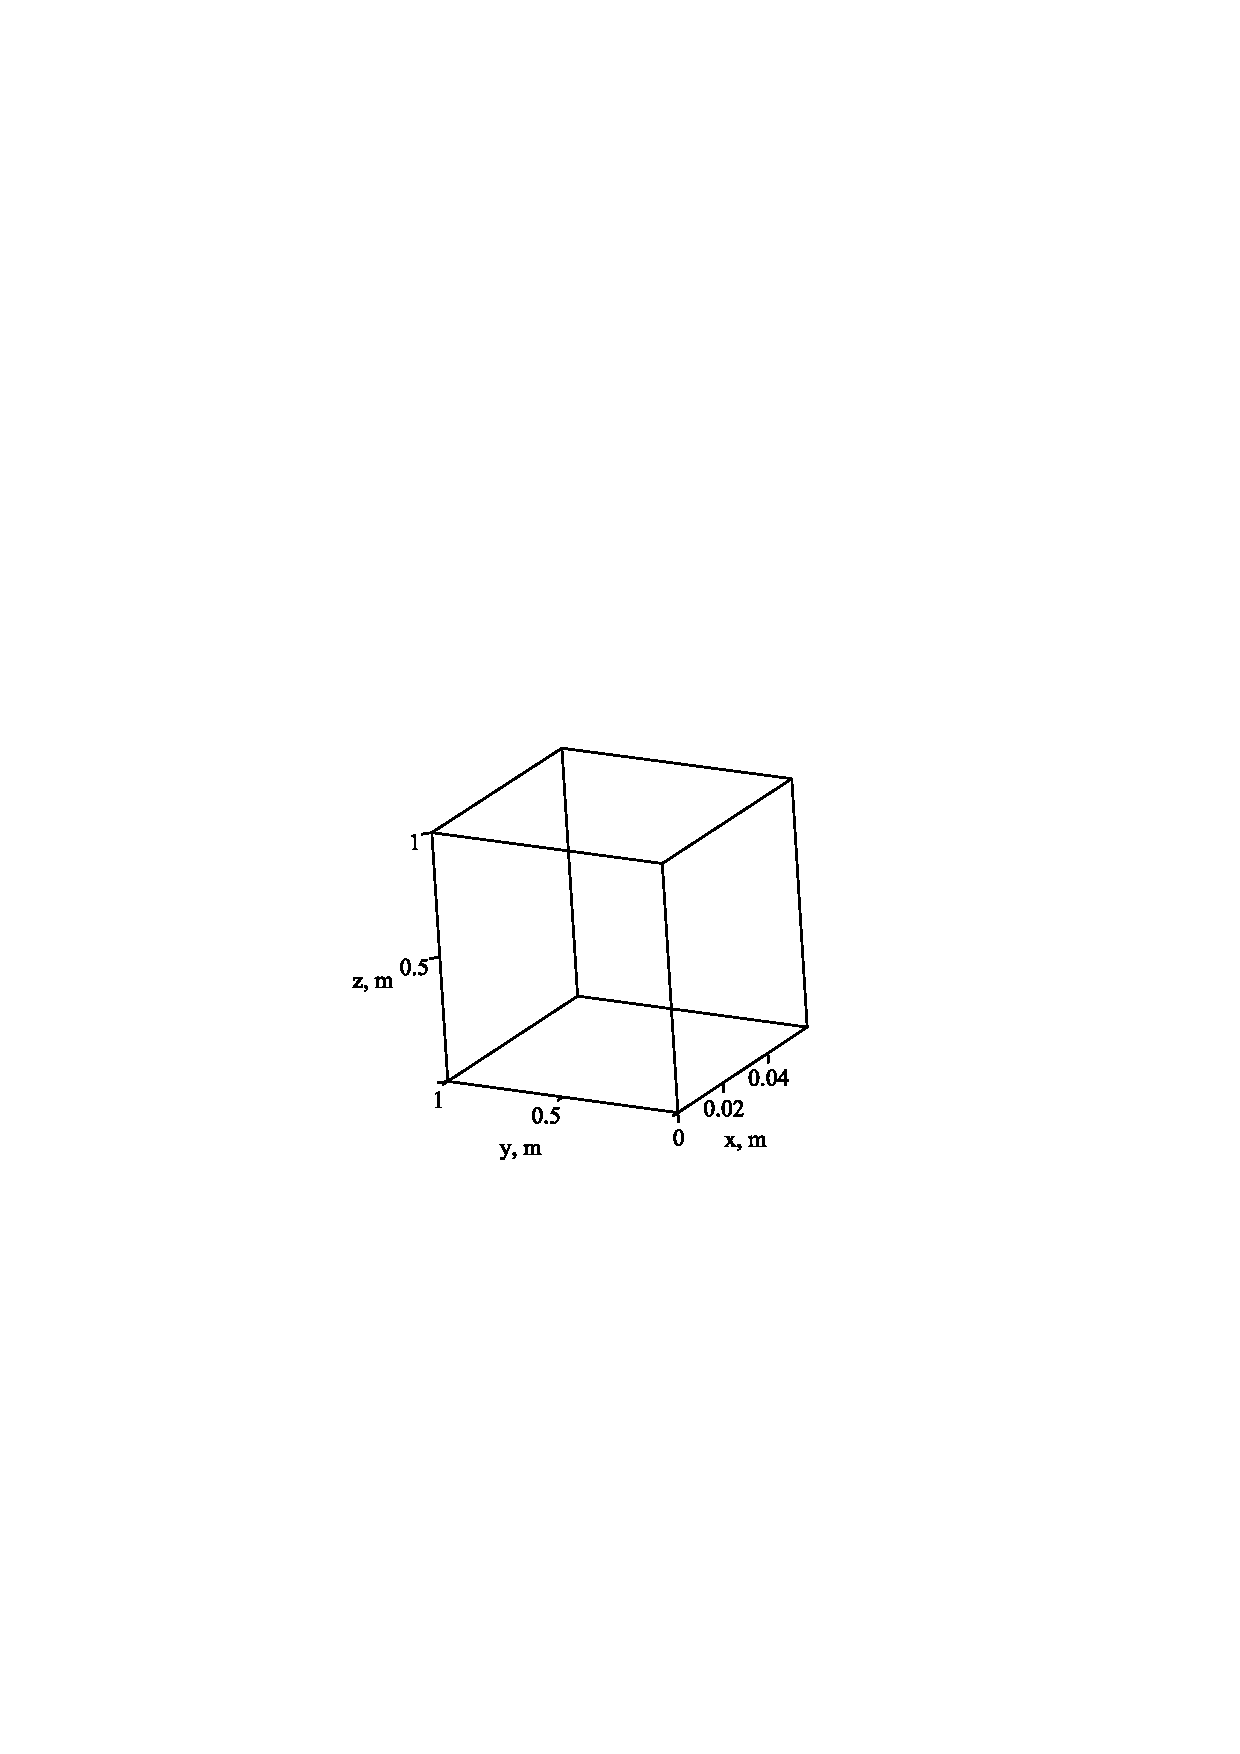
\includegraphics[width=0.95\linewidth]{ModelTrBPR1_.png} \\ а)}
\end{minipage}
\hfill
\begin{minipage}[t]{0.3\linewidth}
	\center{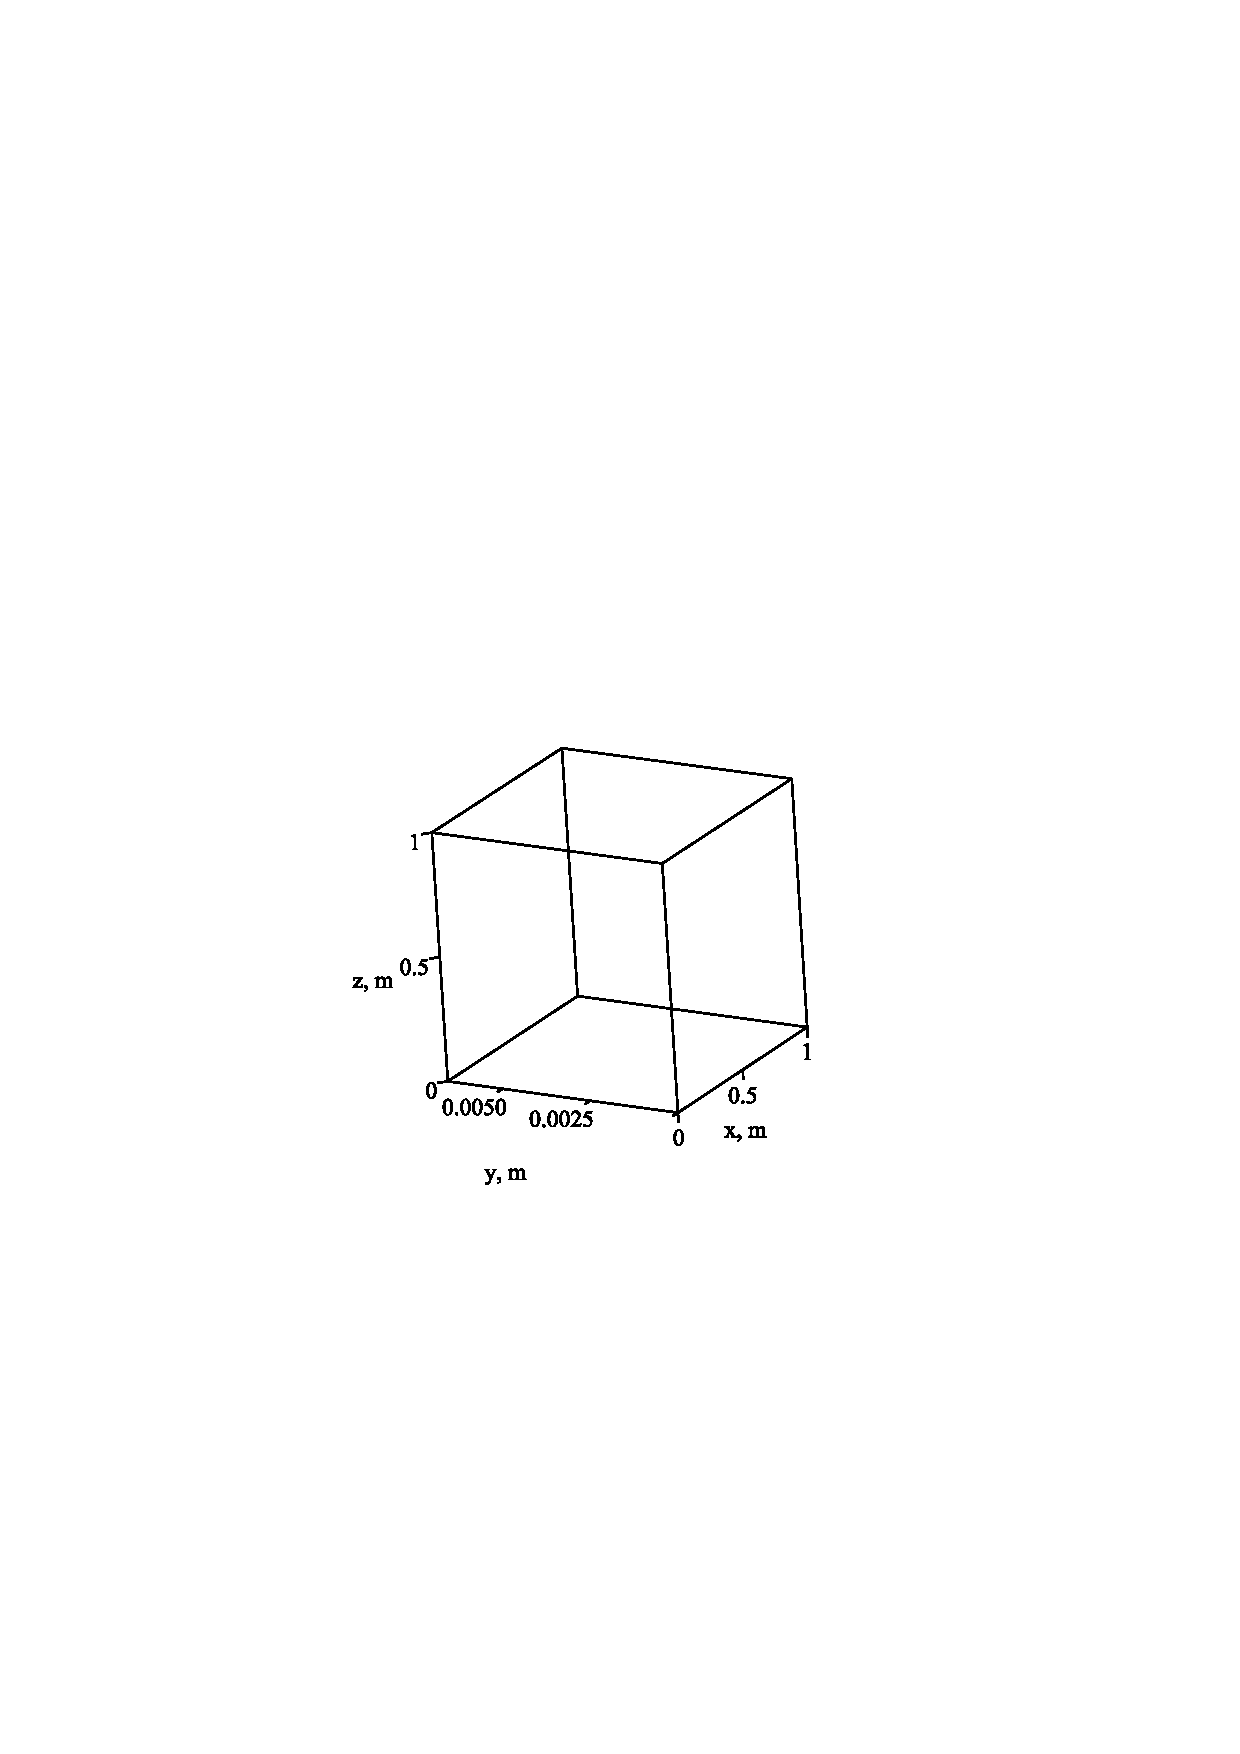
\includegraphics[width=0.95\linewidth]{ModelTrBPR2_.png} \\ б)}
\end{minipage}
\hfill
\begin{minipage}[t]{0.3\linewidth}
	\center{\includegraphics[width=1\linewidth]{ModelTrBPR12_.png} \\ в)}
\end{minipage}


\end{frame}

%\begin{frame}
%\frametitle{Система управления}
%В полученных математических моделях управление роторами задается в виде вектора внутреннего гиростатического момента $\bK$. Для управления отдельным двигателем разработана следующая схема
%
%\begin{figure}[h]
%	\centering
%	\includegraphics[width=0.9\linewidth]{Control_system.png}%
%\end{figure}
%
%Схема управления отдельным двигателем, где $\bK_{set}$ -- вектор внутреннего гиростатического момента; $\bOm_{set}$ -- угловая скорость вращения двигателя; $\hat{\bOm}_{set}$ -- фактическая скорость вращения двигателя; $PWM$ -- широтно-импульсная модуляция, рассчитаная для заданной скорости вращения; $U$ -- напряжение, подаваемое на двигатель; $\varphi$ -- фактическое положение ротора
%
%\end{frame}



\begin{frame}
\frametitle{Экспериментальные исследования}
1.	Вращение пары больших роторов. $K = (2i_1\omega_{max}, 0, 0)$.


	\begin{minipage}[t]{0.3\linewidth}
		\center{\includegraphics[width=0.7\linewidth]{exp11.eps} \\ а)}
	\end{minipage}
	\hfill
	\begin{minipage}[t]{0.3\linewidth}
		\center{\includegraphics[width=0.7\linewidth]{exp12.eps} \\ б)}
	\end{minipage}
	\hfill
	\begin{minipage}[t]{0.3\linewidth}
		\center{\includegraphics[width=0.8\linewidth]{Exp_BPR_1.png} \\ в)}
	\end{minipage}


Положение робота а) в начальный момент времени и б) момент времени t=3 секунды от начала движения; в) теоретическая (сплошная линия) и экспериментальные (штриховые линии) траектории движения безвинтового подводного робота 

\begin{table}[h]
	\centering
	\begin{tabular}{|c|c|c|c|c|c|c|c|}
		\hline
		& $\Delta x$, м & $\Delta y$, м & $\Delta z$, м & $|\br_t|$, м & $\Delta \theta$ & $\Delta \psi$ & $\Delta \varphi$ \\ \hline
		Теория & $0.275$ & $0$ & $0$ & $0.275$ & $ 0^{\circ}$ & $ 0^{\circ}$ & $ 738.2^{\circ}$ \\ \hline
		Эксперимент & $0.115$  & $0.010$ & $0.055$ & $0.128$ & $ 4^{\circ} $ & $ 10^{\circ} $ & $ 121^{\circ} $  \\
		\hline
	\end{tabular}
\end{table}

\end{frame}


\begin{frame}
\frametitle{Экспериментальные исследования}
2.	Вращение одной пары малых роторов. $K = (0, 2i_2\omega_{max}, 0)$. 


	\begin{minipage}[h]{0.3\linewidth}
		\center{\includegraphics[width=0.7\linewidth]{exp21.eps} \\ а)}
	\end{minipage}
	\hfill
	\begin{minipage}[h]{0.3\linewidth}
		\center{\includegraphics[width=0.7\linewidth]{exp22.eps} \\ б)}
	\end{minipage}
	\hfill
	\begin{minipage}[h]{0.3\linewidth}
		\center{\includegraphics[width=0.8\linewidth]{Exp_BPR_2.png} \\ в)}
	\end{minipage}


Положение робота а) в начальный момент времени и б) момент времени t=3 секунды от начала движения; в) теоретическая (сплошная линия) и экспериментальные (штриховые линии) траектории движения безвинтового подводного робота 

\begin{table}[h]
	\centering
	\begin{tabular}{|c|c|c|c|c|c|c|c|}
		\hline
		& $\Delta x$, м & $\Delta y$, м & $\Delta z$, м & $|\br_t|$, м & $\Delta \theta$ & $\Delta \psi$ & $\Delta \varphi$ \\ \hline
		Теория & $0$ & $0.005$ & $0$ & $0.005$ & $ 35^{\circ}$ & $ 0^{\circ}$ & $ 0^{\circ}$ \\ \hline
		Эксперимент & $0.054$  & $0.008$ & $0.068$ & $0.087$ & $ 61^{\circ} $ & $ 62^{\circ} $ & $ 10^{\circ} $  \\
		\hline
	\end{tabular}
\end{table}

\end{frame}


\begin{frame}
\frametitle{Экспериментальные исследования}
3.	Вращение пары больших роторов и одной пары малых роторов. $K = (2i_1\omega_{max}, 2i_2\omega_{max}, 0)$. 

	\begin{minipage}[h]{0.3\linewidth}
		\center{\includegraphics[width=0.7\linewidth]{exp31.eps} \\ а)}
	\end{minipage}
	\hfill
	\begin{minipage}[h]{0.3\linewidth}
		\center{\includegraphics[width=0.7\linewidth]{exp32.eps} \\ б)}
	\end{minipage}
	\hfill
	\begin{minipage}[h]{0.3\linewidth}
		\center{\includegraphics[width=0.8\linewidth]{Exp_BPR_3.png} \\ в)}
	\end{minipage}

Положение робота а) в начальный момент времени и б) момент времени t=3 секунды от начала движения; в) теоретическая (сплошная линия) и экспериментальные (штриховые линии) траектории движения безвинтового подводного робота 

\begin{table}[h]
	\centering
	\begin{tabular}{|c|c|c|c|c|c|c|c|}
		\hline
		& $\Delta x$, м & $\Delta y$, м & $\Delta z$, м & $|\br_t|$, м & $\Delta \theta$ & $\Delta \psi$ & $\Delta \varphi$ \\ \hline
		Теория & $0.275$ & $0$ & $0$ & $0.275$ & $ 35^{\circ}$ & $ 0^{\circ}$ & $ 738.2^{\circ}$ \\ \hline
		Эксперимент & $0.106$  & $0.050$ & $0.053$ & $0.189$ & $ 17^{\circ} $ & $ 92^{\circ} $ & $ 51^{\circ} $  \\
		\hline
	\end{tabular}
\end{table}

%\begin{center}
%	$\Delta x_{exp}=0.106\; \mbox{м}, \; \Delta y_{exp}=0.050\; \mbox{м},\; \Delta z_{exp}=0.053\; \mbox{м}, \;$ \\
%	%\item $|r|=0.129$ м;
%	$\Delta \theta_{exp}=17^{\circ},\; \Delta \psi_{exp}=90^{\circ},\; \Delta \varphi_{exp}=51^{\circ}.$
%\end{center}

\end{frame}


\begin{frame}
\frametitle{Выводы}

\begin{itemize}
	\item	Движение возможно только за счет ускоренного вращения роторов. После достижения максимальной скорости вращения, робот продолжает движение по инерции.
	\item Разгон маховиков до максимальной скорости занимает определенное время, что не учитывается в теоретической модели. %и вносит свой вклад в траекторию движения безвинтового подводного робота.
	\item В теоретической модели используется идеализированная модель вязкости, что так же вносит несоответствия теоретической и реальной траектории движения.
	
	\item	Движение безвинтового подводного робота сопровождается образованием вихревых структур. Обеспечить безвихревое движение крайне затруднительно.
	
	\item Подобную схему и алгоритмы управления в качестве практического применения можно использовать для реализации различных маневров (например, разворот на месте) в управлении подводными роботами.
	
	\item \textbf{Модель качественно описывает движение, но на количественное согласование влияет точность определения большого количества параметров. Движение возможно, однако, его эффективность не высока.}
\end{itemize}

\end{frame}

%\begin{frame}
%\frametitle{Переход}
%
%Ассиметрия тела
%периодическое управление
%Вихри помогают, оболочка с участием вихрей - острая кромка.
%Наводный для простоты.
%
%
%
%
%\end{frame}


%\section{Недеформируемый водный робот с внутренним ротором}
%
%\begin{frame}[plain, noframenumbering]
%\begin{center}
%	\Huge
%	Недеформируемый водный робот с внутренним ротором
%\end{center}
%\end{frame}

%\begin{frame}
%\frametitle{Краткая история}
%
%Краткая история
%
%\end{frame}

\begin{frame}
\frametitle{Недеформируемый водный робот с острой кромкой}

\begin{figure}[!ht]
	\centering
	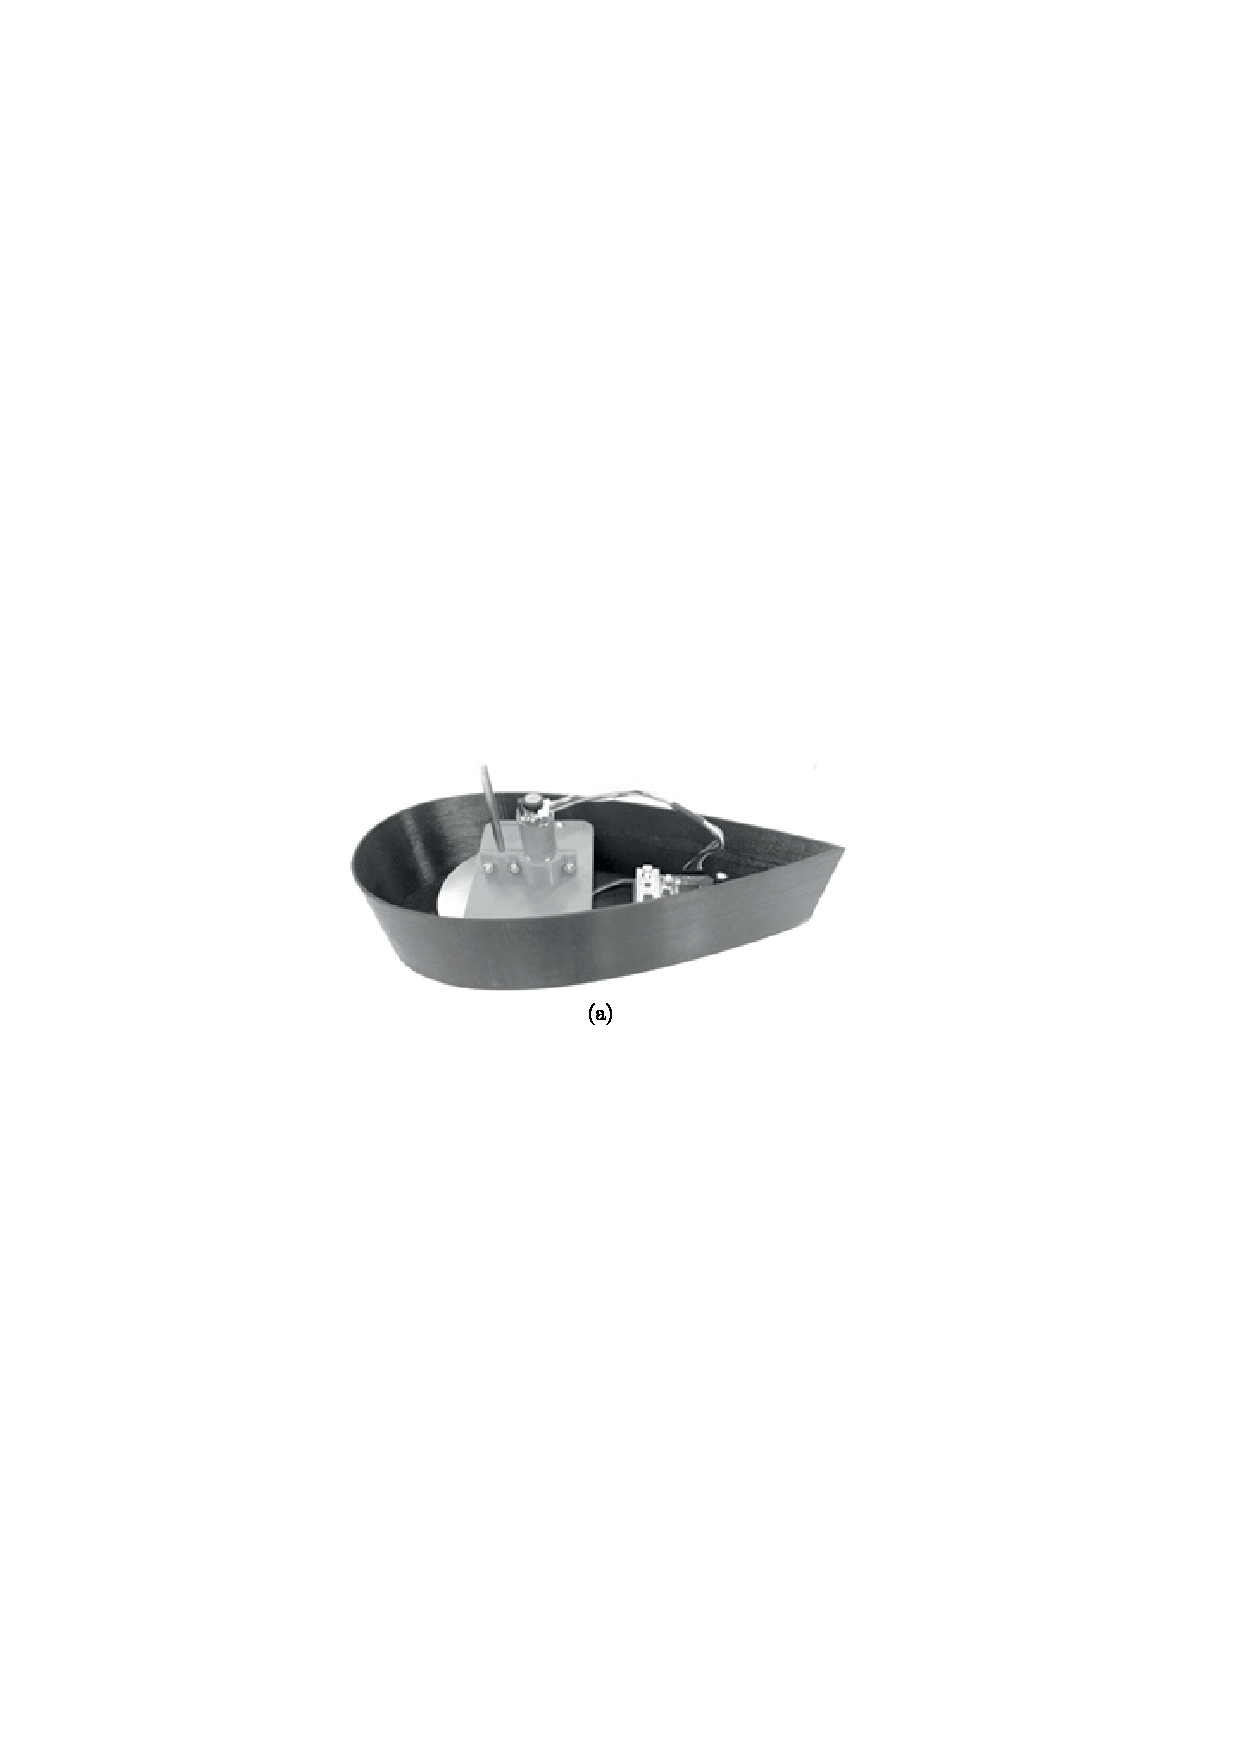
\includegraphics[height=25mm]{Photo_NACA1.png} \hspace{10mm} \includegraphics[height=25mm]{Kinematic_Scheme2.eps}
\end{figure}

\begin{table}[h]
	\centering
	\begin{tabular}{|l|c|c|}
		\hline
		Параметр & Обозначение & Значение \\ \hline
		Масса робота & $m$ & $0.905$ кг \\
		Осевой момент инерции робота & $I_0$ & 0.00844 кг$\cdot$м$^2$ \\
		Масса ротора & $m_r$ &  0.327 кг \\
		Осевой момент инерции ротора & $I_r$ & 0.00058 кг$\cdot$м$^2$ \\
		\hline
	\end{tabular}
	%\caption{Значения параметров созданного робота}
	\label{tab1}
\end{table}
\centering{Значения параметров созданного робота}

\end{frame}


\begin{frame}
\frametitle{Система управления}
Для управления безвинтовым недеформируемым рыбоподобным надводным роботом была разработана система управления, структурная схема которой представлена на рисунке

\begin{figure}[!h]
\centering
\includegraphics[width=0.8\linewidth]{ControlSystem.eps}
\end{figure}

\end{frame}

\begin{frame}%[allowframebreaks]
\frametitle{Математическая модель. Уравнения движения}
%\qquad Для описания движения робота рассмотрим систему представленную на рисунке:

\begin{minipage}[t]{0.35\linewidth}
	\begin{figure}[h]
		\begin{center}
			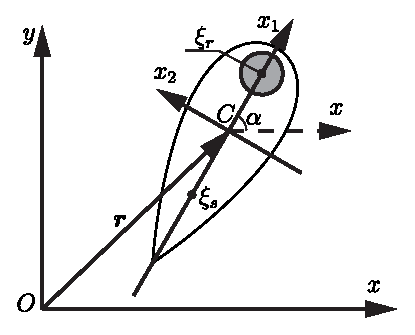
\includegraphics[width=0.9\linewidth]{coords.eps}
		\end{center}
	\end{figure}	
\end{minipage}
\hfill
\begin{minipage}[t]{0.63\linewidth}
	$Oxy$ -- неподвижная система координат,
	
	$Cx_1x_2$ -- подвижная система координат.%, жестко связанная с телом.
	
	$\bs r = (x,\, y)$ радиус-вектор точки $C$, определяющий положение системы.
	
	Угол $\alpha$ определяет ориентацию системы.
	
	Справедливы следующие кинематические соотношения:
	\vspace{-3mm}
	\begin{gather*}	
	%\begin{gathered}
	\dot{x} = v_1 \cos\alpha - v_2 \sin\alpha,\quad \dot{y} = v_1 \sin\alpha + v_2 \cos\alpha, \\
	\dot{\alpha} = \omega.
	%\end{gathered}
	\end{gather*}
	
\end{minipage}	

Описание движения -- уравнения Ньютона-Эйлера в подвижных осях: %, жестко связанных с телом:
\begin{gather*}
\begin{gathered}
m \dot{v}_1 = m v_2 \omega + f_1 (v_1,\, v_2,\, \omega,\, \dot{v}_1,\, \dot{v}_2,\, \dot \omega),\quad m \dot{v}_2 = -m v_1 \omega + f_2 (v_1,\, v_2,\, \omega,\, \dot{v}_1,\, \dot{v}_2,\, \dot \omega),\\
I \dot{\omega} = g (v_1,\, v_2,\, \omega,\, \dot{v}_1,\, \dot{v}_2,\, \dot \omega),
\end{gathered}\label{eq.NE}
\end{gather*}

Для определения вида $ f_1 $, $ f_2 $ и $ g $ воспользуемся уравнениями Кирхгофа, дополнеными слагаемыми, описывающими вязкое сопротивление:% \cite{Borisov_et_al_2016}:
\begin{equation*}
\begin{gathered}
\der{}{t} \pder{T}{v_1} = \omega \pder{T}{v_2} - c_1 v_1 |v_1|,\quad \der{}{t} \pder{T}{v_2} = - \omega \pder{T}{v_1} - c_2 v_2 |v_2|,\\
\der{}{t} \pder{T}{\omega} = v_2 \pder{T}{v_1} - v_1 \pder{T}{v_2} - c_3 \omega |\omega|,
\end{gathered}\label{eq.kirchhoff}
\end{equation*}
%где $T$ --- кинетическая энергия системы (корпус + ротор + жидкость); $c_1$, $c_2$, $c_3$ --- коэффициенты сопротивления.



\end{frame}



%\begin{frame}
%\frametitle{Математическая модель}
%
%	\begin{itemize}
%	
%		%где $m$, $I$ --- масса и момент инерции робота соответственно, $f_1$, $f_2$ --- проекции силы реакции жидкости на подвижные оси, связанные с телом, $g$ --- момент силы реакции жидкости.
%		\item Движение твердого тела в идеальной жидкости при нулевой циркуляции описывается уравнениями Кирхгофа. % их необходимо дополнить слагаемыми, описывающими вязкое трение \cite{Borisov_et_al_2016}:
%		\begin{equation*}
%		\begin{gathered}
%		\der{}{t} \pder{T}{v_1} = \omega \pder{T}{v_2} - c_1 v_1 |v_1|,\quad \der{}{t} \pder{T}{v_2} = - \omega \pder{T}{v_1} - c_2 v_2 |v_2|,\\
%		\der{}{t} \pder{T}{\omega} = v_2 \pder{T}{v_1} - v_1 \pder{T}{v_2} - c_3 \omega |\omega|,
%		\end{gathered}\label{eq.kirchhoff}
%		\end{equation*}
%		где $T$ --- кинетическая энергия системы (корпус + ротор + жидкость), $c_1$, $c_2$, $c_3$ --- коэффициенты сопротивления.
%		
%		Кинетическая энергия системы с точностью до некоторой функции времени имеет вид
%		\begin{gather*}
%		T = \frac{1}{2}(m + \lambda_{11}) v_1^2 + \frac{1}{2}(m + \lambda_{22}) v_2^2 + \frac{1}{2} (I + \lambda_{33}) \omega^2 + \lambda_{23} v_2\omega + \omega k(t),\label{eq.T}\\
%		\begin{gathered}
%		m = m_s + m_r,\quad
%		I = I_s + m_s \xi_s^2 + I_r + m_r \xi_r^2,\quad k(t) = I_r \Omega(t),
%		\end{gathered}\notag
%		\end{gather*}
%	\end{itemize}
%
%\end{frame}


\begin{frame}
\frametitle{Математическая модель. Уравнения движения}

Кинетическая энергия системы с точностью до некоторой функции времени имеет вид:
\begin{gather*}
T = \frac{1}{2}(m + \lambda_{11}) v_1^2 + \frac{1}{2}(m + \lambda_{22}) v_2^2 + \frac{1}{2} (I + \lambda_{33}) \omega^2 + \lambda_{23} v_2\omega + \omega k(t),\label{eq.T}\\
\begin{gathered}
m = m_s + m_r,\quad
I = I_s + m_s \xi_s^2 + I_r + m_r \xi_r^2,\quad k(t) = I_r \Omega(t),
\end{gathered}\notag
\end{gather*}

Полная система уравнений рассматриваемой системы может быть записана в следующей форме:
		\begin{equation*}
		\begin{split}\label{eq.dyn}
		(m + \lambda_{11}) \dot{v}_1 = {} & {} (m + \lambda_{22}) v_2 \omega + \lambda_{23}\omega^2 - c_1 v_1 |v_1|,\\
		(m + \lambda_{22}) \dot{v}_2 + \lambda_{23} \dot{\omega} = {} & {} - (m + \lambda_{11}) v_1 \omega - c_2 v_2 |v_2|,\\
		\lambda_{23,l}\dot{v}_2 + (I + \lambda_{33}) \dot{\omega} = {} & {} (\lambda_{11} - \lambda_{22}) v_1 v_2 - \lambda_{23,r} v_1\omega - c_3 \omega |\omega| - \dot{k}(t),
		\end{split}
		\end{equation*}
		\begin{equation*}
		\dot{x} = v_1 \cos\alpha - v_2 \sin\alpha,\quad \dot{y} = v_1 \sin\alpha + v_2 \cos\alpha,\quad \dot{\alpha} = \omega.
		\end{equation*}

	
	
	 %Сравнивая уравнения \eqref{eq.dyn} с уравнениями Ньютона-Эйлера \eqref{eq.NE}, запишем 
	 Выражения для сил $f_1$, $f_2$ и момента $g$:
	\begin{gather*}
	\begin{gathered}\label{eq.forceTorque}
	f_1 = - \lambda_{11}\dot{v}_1 + \lambda_{22} v_2 \omega + \lambda_{23}\omega^2 - c_1 v_1 |v_1|, \quad
	f_2 = - \lambda_{22} \dot{v}_2 - \lambda_{23} \dot{\omega} - \lambda_{11} v_1 \omega - c_2 v_2 |v_2|,\\
	g = -\lambda_{23}\dot{v}_2 - \lambda_{33} \dot{\omega} + (\lambda_{11} - \lambda_{22}) v_1 v_2 - \lambda_{23} v_1\omega - c_3 \omega |\omega| - \dot{k}(t).
	\end{gathered}
	\end{gather*}
	%где коэффициенты $\lambda_{ij}$ и $c_i$ подлежат определению, а $\dot{k}(t)$ --- определяется управляющим воздействием на ротор.


\end{frame}




\begin{frame}
\frametitle{Закон изменения угловой скорости ротора}

	В общем случае, зависимость угловой скорости ротора от времени будет иметь характерные переходные интервалы, соответствующие разгону и торможению 
	
		\scriptsize 
		\vspace{-4mm}
		\begin{equation*}
		\omega_r(t) =
		\begin{cases}
		
		\omega_1 & t \in \left[ nT;  nT + t_1 \right] ,\\
		
		\frac{(\omega_2 - \omega_1)(t-nT)}{t_2} - \frac{(\omega_2 - \omega_1)(t_1+t_2)}{t_2} + \omega_2 & t \in \left[ nT + t_1;  nT + t_1+t_2 \right], \\
		
		\omega_2 & t \in \left[ nT + t_1+t_2;  nT + t_1+t_2+t_3 \right] ,\\
		
		\frac{(\omega_1 - \omega_2)(t-nT)}{t_4} - \frac{(\omega_1 - \omega_2)(t_1+t_2+t_3+t_4)}{t_4} + \omega_1 &t \in \left[ nT + t_1 + t_2+t_3;  nT + t_1+t_2+t_3+t_4 \right] ,
		
		\end{cases}
		\label{omegaRotorGeneral}
		\end{equation*}
		
		\small
		где $n \in \mathbf{N}$, $T$ -- период управляющего воздействия; $ \omega_1, \omega_2 $ -- амплитуды угловой скорости вращения ротора по часовой стрелке и против часовой стрелки соответственно; $t_1, t_2, t_3, t_4$ -- задают продолжительность по времени характерных интервалов угловой скорости вращения ротора. 
		
			%\framebreak
		
		%Графически данная зависимость приведена на рисунке
		
		\begin{minipage}[t]{0.47\linewidth}
			\begin{figure}[!ht]
				\centering
				\includegraphics[height=33mm]{ControlAction.eps}
			\end{figure}
			
		\end{minipage}	
		\hfill
		\begin{minipage}[t]{0.47\linewidth}
			\begin{figure}[!ht]
				\centering
				\includegraphics[height=33mm]{ControlActionEpsilon.eps}
			\end{figure}
		\end{minipage}	
%		\begin{figure}[!ht]
%			\centering
%			\includegraphics[width=0.4\linewidth]{ControlAction.eps}
%		\end{figure}
	
	
\end{frame}

%\begin{frame}
%\frametitle{Результаты моделирования}
%
%Моделирование различных управляющих воздействий
%
%\end{frame}



\begin{frame}
\frametitle{Методика проведения экспериментов}

	\begin{itemize}
		\item Эксперименты проводились в бассейне размерами $2 \times 1.2$ метра. 
		\item Траектория движения робота и его ориентация в процессе движения восстанавливались с помощью системы захвата движения фирмы Vicon, включающей 7 камер, расположенных по периметру бассейна. 
		\item Типовая траектория движения, восстановленная с помощью системы захвата движения и наложенная на кадр с видеозаписи в бассейне
		
		\begin{figure}[!h]
			\centering
			\includegraphics[width=0.8\linewidth]{Frame1col.png}
		\end{figure}
	\end{itemize}



\end{frame}


\begin{frame}
\frametitle{Движение вдоль прямой}

1. $t_1=t_3$, $ t_2 = t_4$; \quad $ \omega_1 = \omega_{max} $, $ \omega_2 = -\omega_{max} $.

\begin{minipage}[t]{0.3\linewidth}
	\begin{figure}[!ht]
		\centering
		\includegraphics[width=1\linewidth]{ControlActionLine.eps}
	\end{figure}	
\end{minipage}
\hfill
\begin{minipage}[t]{0.68\linewidth}
	\begin{figure}[!ht]
		\centering
		\includegraphics[width=1\linewidth]{AllTrajectories_new.eps}
	\end{figure}
\end{minipage}	
	
2. 	$t_1=t_3$, $ t_2 = t_4$, $ T=2 $ с.; \quad $ \omega_1 - \omega_2 = const$

\begin{minipage}[h]{0.47\linewidth}
	\center{\includegraphics[width=0.6\linewidth]{ControlActionPlots3.eps} }
\end{minipage}
\hfill
\begin{minipage}[h]{0.47\linewidth}
	\center{\includegraphics[width=0.6\linewidth]{Plots3.eps}}
\end{minipage}


\end{frame}



\begin{frame}
\frametitle{Движение вдоль окружности}

1. $t_1 \neq t_3$, $t_2 = t_4$ с; \quad	$ \omega_1 = \omega_{max} $, $ \omega_2 = -\omega_{max} $; \quad $ k_1 = t_3 / t_1 $
		
	
	\begin{minipage}[t]{0.47\linewidth}
	{Угловая скорость ротора}
			\center{\includegraphics[width=0.7\linewidth]{ControlActionCircle.eps}}
	\end{minipage}
	\hfill
	\begin{minipage}[t]{0.47\linewidth}
		{Траектория движения робота}
		\center{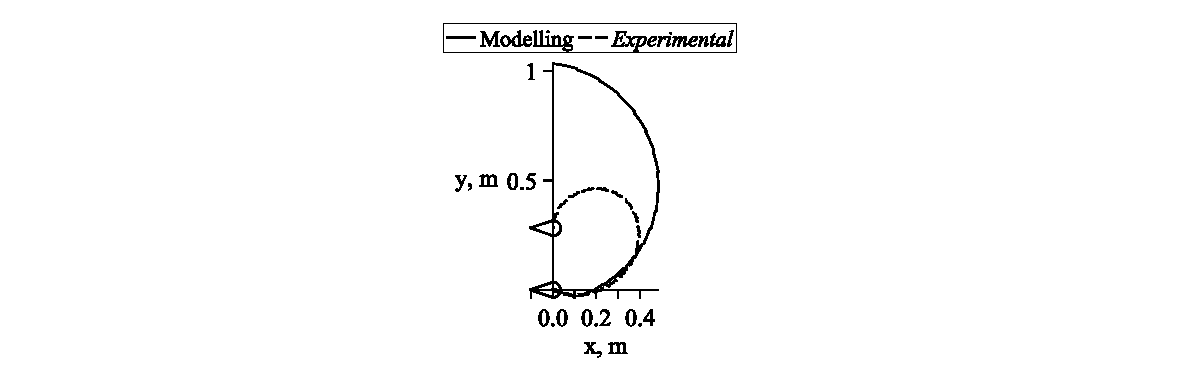
\includegraphics[width=0.35\linewidth]{xyCircleWmax.eps}}
	\end{minipage}

\vspace{4mm}

2. $t_1 = t_3$, $t_2 \neq t_4$ с; \quad $ \omega_1 = \omega_{max} $, $ \omega_2 = -\omega_{max} $ \quad $ k_2 = t_2 / t_4 $

\begin{minipage}[t]{0.47\linewidth}
	{Угловая скорость ротора}
	\center{\includegraphics[width=0.7\linewidth]{ControlActionOur1.eps}}
\end{minipage}
\hfill
\begin{minipage}[t]{0.47\linewidth}
	{Траектория движения робота}
	\center{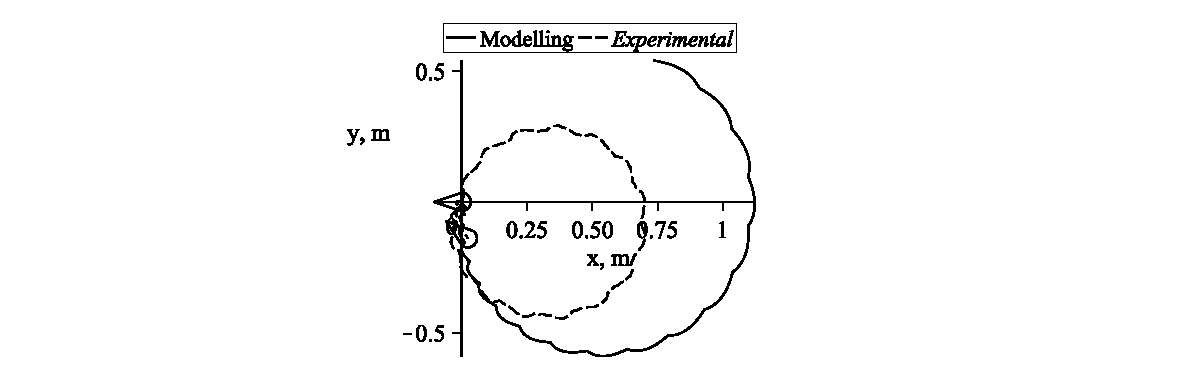
\includegraphics[width=0.5\linewidth]{xyCircleOur.eps}}
\end{minipage}

\end{frame}


\begin{frame}
\frametitle{Движение вдоль окружности}

Зависимость радиуса траектории движения робота от $k_1 ={t_3}/{t_1}$ при эксперименте (штриховая линия) и моделировании (сплошная линия) построенная по экспериментам при $k_1 = 2, 3, 5, 10$

\begin{figure}[!ht]
	\centering
	\includegraphics[width=0.5\linewidth]{kRDependence+Theor_T=3,W=max.eps}
\end{figure}
	
Зависимость радиуса траектории движения робота от $k_2 = {t_2}/{t_4}$ при эксперименте (штриховая линия) и моделировании (сплошная линия) построенная по экспериментам при $k_2 = 10, 20, 30, 40$

\begin{figure}[!ht]
	\centering
	\includegraphics[width=0.5\linewidth]{nROur.eps}
\end{figure}		
%\begin{minipage}[t]{0.47\linewidth}
%	{Зависимость радиуса траектории движения робота от $k_1 = \frac{t_3}{t_1}$ при эксперименте (штриховая линия) и моделировании (сплошная линия) построенная по экспериментам при $k_1 = 2, 3, 5, 10$}
%	\center{\includegraphics[width=0.9\linewidth]{kRDependence+Theor_T=3,W=max.eps}}
%\end{minipage}
%\hfill
%\begin{minipage}[t]{0.47\linewidth}
%	{Зависимость радиуса траектории движения робота от $k_2 = \frac{t_2}{t_4}$ при эксперименте (штриховая линия) и моделировании (сплошная линия) построенная по экспериментам при $k_2 = 10, 20, 30, 40$}
%	\center{\includegraphics[width=1.05\linewidth]{nROur.eps}}
%\end{minipage}

\end{frame}


\begin{frame}
\frametitle{Выводы}
\begin{itemize}
	\item Рассматриваемая теоретическая модель управляемого движения водного робота качественно правильно описывает его движение. Cимметричное управляющее воздействие -- движение вдоль прямой. Асимметричное управляющее воздействие -- движение вдоль окружности.
	
	\item Сдвиг управляющего воздействия $\omega(t) \rightarrow \omega_0 + \omega(t)$ не влияет на форму траектории. На размер и форму траектории движения влияет асимметрия управляющего воздействия на его периоде.
	
	\item Количественного согласования результатов моделирования и экспериментов можно достичь для конкретных тестов, проводя перерасчет коэффициентов под конкретные экспериментальные данные.
	
	\item Комбинируя описанные маневры, можно двигаться по сложной траектории.
	
	%\item Рассматриваемая теоретическая модель управляемого движения водного робота качественно правильно  описывает его движение вдоль окружности, которое реализуется асимметричным на периоде управляющим воздействием.
	%\item На размер и форму траектории движения влияет асимметрия управляющего воздействия на его периоде. Изменение направления движения -- поворот, может быть реализован либо при изменении продолжительности интервала вращения с постоянной угловой скоростью, либо вращением ротора по и против часовой стрелки с различными угловыми ускорениями.
	%\item Количественного согласования результатов моделирования и экспериментов, как и в при движении вдоль прямой, можно достичь для конкретных тестов, проводя перерасчет коэффициентов под конкретные экспериментальные данные, полученные при движении вдоль окружности.
\end{itemize}

\end{frame}


\begin{frame}
\frametitle{Экспериментальные исследования. Движение вдоль сложных траекторий}


	{Управление для слалома}
	\centering
	\includegraphics[width=0.7\linewidth]{ControlActionComplexTr.eps}

	{Траектория движения робота при эксперименте (штриховая линия) и моделировании (сплошная линия)}
	\centering
	\includegraphics[width=0.7\linewidth]{ComplexTr.eps}


\end{frame}

%\begin{frame}
%\frametitle{Экспериментальные исследования. Видео.}
%
%\begin{figure}[ht]
%	%\vspace{-7pt}
%	%\hspace*{-28.5pt}
%	\includemovie[
%	%autoplay,
%	%repeat,
%	%poster=ComplexTr1.png,
%	inline=false,
%	text={Video}
%	]{\textwidth}{0.6\textwidth}{ComplexTr1.avi}
%\end{figure}

%\movie[width=0.5\textwidth]{\includegraphics[width=0.5\textwidth]{ComplexTr1.png}}{123.mp4}
%\includemedia[activate=onclick, width=0.5\textwidth]{\includegraphics{ComplexTr1.png}}{123.mp4}
%\includemedia[
%activate=pageopen,
%width=1280pt,height=720pt,
%addresource=123.mp4,
%flashvars={
%	source=123.mp4}
%]{}{VPlayer.swf}

%\end{frame}



\begin{frame}
\frametitle{Заключение}
\begin{itemize}
	\item Адекватность математической модели с точки зрения качественного описания движения.
	\item Количественное отклонение может быть минимизировано уточнением коэффициентов модели движения для различных движений.
	%\item Основная причина отклонения результатов моделирования -- рассчет коэффициентов модели на основании экспериментальных  данных, полученных при симметричном управляющем воздействии с $T = 1 $ c.
	\item Для повышения совпадения результатов моделирования и экспериментов можно обеспечить более точное совпадение формы углового ускорения в моделировании и при эксперименте.
\end{itemize}

Зависимость угловой скорости ротора и углового ускорения ротора от времени при эксперименте (штриховая линия) и моделировании (сплошная линия)

\begin{minipage}[t]{0.47\linewidth}
	\center{\includegraphics[width=1\linewidth]{OmegaT1Meandr.eps}}
\end{minipage}
\hfill
\begin{minipage}[t]{0.47\linewidth}
	\center{\includegraphics[width=1\linewidth]{EpsilonT1Meandr.eps}}
\end{minipage}

\end{frame}



%%%%%%%%%%%%%%%%%%%%%%%%%%%%%%%%%%%%%%%%%%%%%%%%%%%%%%%%%%%%%%%%%%%%%%%%%%%%%%%%%%%%%%%%%%%%
